%@TheDoctorRAB
%standard white paper/preproposal format
%
%%%%%
%
%REFERENCES
%
%neup.bst - numbered citations in order of appearance, short author list with et al in reference section
%nsf.bst - numbered citations in order of appearance, full author list in references section
%standard.bst - citations with author last name with et al for more than 2 authors; full author list in references section
%ans.bst is for ANS only. 
%
%author = {Lastname, Firstname and Lastname, Firstname and Lastname, Firstname} for all bst formats
%bst renders the author list itself
%
%author = {{Nuclear Regulatory Commission}} if the author is an organization, institution, etc., and not people
%
%title = {{}} for all
%
%for all - use \citep{-} - [1] or (Borrelli, 2021) in the text
%standard.bst \cite{-} - Borrelli (2021) in the text
%standard.bst lists references alphabetically
%the rest list numerically
%
%
%%% slides 
%
%\citep{xxxnna} where the citation should go
%\blfootnote{\fontsize\cite{xxxnna}\fontsize\bibentry{xxxnna}} before \end{frame}
%
%
%%%%%

%%%%% presentation settings
\documentclass[aspectratio=1610,pdftex,dvipsnames,compress,xcolor={dvipsnames}]{beamer}
\usetheme{Boadilla}
\usecolortheme{seahorse}
\beamertemplatenavigationsymbolsempty
\addtobeamertemplate{footnote}{\hskip -2em}{} %pushes footnote to margin
\setbeamerfont{title}{series=\bfseries}
\setbeamertemplate{page number in head/foot}[framenumber] %just gives slide number; comment out for 1/7, 2/7...
\definecolor{BackGround}{RGB}{255,250,240}
\setbeamercolor{background canvas}{bg=BackGround}
%%%%%


%%%%% general 
%\documentclass[11pt,a4paper]{article}
%\usepackage[lmargin=1in,rmargin=1in,tmargin=1in,bmargin=1in]{geometry}
\usepackage[pagewise]{lineno} %line numbering
\usepackage{setspace}
\usepackage{ulem} %strikethrough - do not \sout{\cite{}}
\usepackage{graphicx}
\usepackage{mypythonhighlight,verbatim}
\usepackage{filecontents}
\usepackage{tablefootnote}
\usepackage{footnotehyper}
\usepackage{float}
%\usepackage{subfig}
\usepackage[yyyymmdd]{datetime} %date format
\renewcommand{\dateseparator}{.}
\graphicspath{{img/}} %path to graphics
\setcounter{secnumdepth}{5} %set subsection to nth level
\usepackage{needspace}
\usepackage[stable,hang,flushmargin]{footmisc} %footnotes in section titles and no indent; standard.bst
\usepackage[inline]{enumitem}
\setlist[itemize]{label=\textbullet}
\usepackage{boldline}
\usepackage{makecell}
\usepackage{booktabs}
\usepackage{amssymb}
\usepackage{gensymb}
\usepackage{amsmath,nicefrac}
\usepackage{physics}
\usepackage{lscape}
\usepackage{array}
\usepackage{chngcntr}
\usepackage{hyperref}
\hypersetup{colorlinks,linkcolor=black,citecolor=black,urlcolor=blue} 
%\usepackage{sectsty}
\usepackage{textcomp}
\usepackage{lastpage}
\usepackage{xargs} %for \newcommandx
\usepackage[colorinlistoftodos,prependcaption,textsize=tiny]{todonotes} %makes colored boxes for commenting
\usepackage{soul}
\usepackage{color}
\usepackage{marginnote}
\usepackage[figure,table]{totalcount}
\usepackage[capitalise]{cleveref}
\usepackage{microtype} %improves typography for pdf
\usepackage[pdftex,dvipsnames]{colortbl} %change font color
%%%%%


%%%%% tikz
\usepackage{pgf}
\usepackage{tikz} % required for drawing custom shapes
\usetikzlibrary{shapes,arrows,automata,trees}
%%%%%


%%%%% fonts
\usepackage{times}
%arial - uncomment next two lines
%\usepackage{helvet}
%\renewcommand{\familydefault}{\sfdefault}
%%%%%


%%%%% references
%\usepackage[round,semicolon]{natbib} %for (Borrelli 2021; Clooney 2019) - standard.bst 
\usepackage[numbers,sort&compress]{natbib} %for [1-3] - nsf.bst, neup.bst
\setlength{\bibsep}{7pt} %sets space between references
%\renewcommand{\bibsection}{} %suppresses large 'references' heading
%\renewcommand\bibpreamble{\vspace{\baselineskip}} %sets spacing after heading if not using default references heading
%%%%%


%%%%% tables and figures
\usepackage{longtable} %need to put label at top under caption then \\ - use spacing
\usepackage{tablefootnote}
\usepackage{tabularx}
\usepackage{multirow}
\usepackage{tabto} %general tabbed spacing
\usepackage{pdfpages}
\usepackage{wrapfig} %wraps figures around text
\setlength{\intextsep}{0.00mm}
\setlength{\columnsep}{1.00mm}
\usepackage[singlelinecheck=false,labelfont=bf]{caption}
\usepackage{subcaption}
\captionsetup[table]{justification=justified,skip=5pt,labelformat={default},labelsep=period,name={Table}} %sets a space after table caption
\captionsetup[figure]{justification=justified,skip=5pt,labelformat={default},labelsep=period,name={Figure}} %sets space above caption, 'figure' format
\captionsetup[wrapfigure]{justification=centering,aboveskip=0pt,belowskip=0pt,labelformat={default},labelsep=period,name={Fig.}} %sets space above caption, 'figure' format
\captionsetup[wraptable]{justification=centering,aboveskip=0pt,belowskip=0pt,labelformat={default},labelsep=period,name={Table}} %sets space above caption, 'figure' format
%%%%%


%%%%% watermark
%\usepackage[firstpage,vpos=0.63\paperheight]{draftwatermark}
%\SetWatermarkText{\shortstack{DRAFT\\do not distribute}}
%\SetWatermarkScale{0.20}
%%%%%


%%%%% cross referencing files
%\usepackage{xr} %for revisions - will cross reference from one file to here
%\externaldocument{/path/to/auxfilename} %aux file needed
%%%%%


%%%%% toc and glossaries
\usepackage[toc,title]{appendix}
\usepackage[acronym,nomain,nonumberlist]{glossaries}
\makenoidxglossaries
%\usepackage{titlesec,titletoc}
%\renewcommand{\thepart}{ARTICLE \Roman{part}} %puts the label into the command so \thelabel will carry through
%\renewcommand{\thesection}{\arabic{section}} %puts the label into the command so \thelabel will carry through
%\titleformat{\part}{\normalfont\large\bfseries}{\thepart}{}{}[]
%\titlespacing*\part{0pt}{0.95\baselineskip}{0.75\baselineskip}
%\titleformat{\section}[runin]{\normalfont\large\bfseries}{\thesection}{-1em}{}[.]
%\titlespacing*\section{0pt}{0.65\baselineskip}{0.55\baselineskip}
%\titleformat{\subsection}[runin]{\normalfont\normalsize\bfseries}{\thesubsection}{-1em}{}[.]
%\titlespacing*\subsection{0pt}{0.50\baselineskip}{0.35\baselineskip}
%\titleformat{\paragraph}[runin]{\normalfont\normalsize\bfseries\itshape}{\theparagraph}{-1em}{}[.]
%\titlespacing*\paragraph{0pt}{0.45\baselineskip}{0.25\baselineskip}
%\titleformat{\subparagraph}[runin]{\normalfont\normalsize\itshape}{\thesubparagraph}{-1em}{}[.]
%\titlespacing*\subparagraph{0pt}{0.40\baselineskip}{0.25\baselineskip}
%\titleformat{\paragraph}[hang]{\normalfont\normalsize\bfseries}{\theparagraph}{5pt}{}[]
%\titlespacing*\paragraph{0pt}{0.50\baselineskip}{0.25\baselineskip}
%\titleformat{\subparagraph}[runin]{\normalfont\normalsize\itshape}{\thesubparagraph}{-1em}{}[.]
%\titlespacing*\subparagraph{0pt}{0.40\baselineskip}{0.20\baselineskip}
%%%%%


%%%%% editing
\newcommand{\edit}[1]{\textcolor{blue}{#1}} %shortcut for changing font color on revised text
\newcommand{\fn}[1]{\footnote{#1}} %shortcut for footnote tag
\newcommand*\sq{\mathbin{\vcenter{\hbox{\rule{.3ex}{.3ex}}}}} %makes a small square as a separator $\sq$
%\newcommand{\sk}[1]{\sout{#1}} %shortcut for default strikethrough - do not sk through citep
\newcommand\sk{\bgroup\markoverwith{\textcolor{red}{\rule[0.5ex]{1pt}{1pt}}}\ULon} %strikethrough with red line; not in \section{}
%\st{} does strikethrough using soul package but does not like acronyms
\newcommand{\blucell}{\cellcolor{aliceblue}} %use to shade in table cell
\newcommand{\grycekk}{\cellcolor{lightgray}} %use to shade in table cell
\newcommand{\whicell}{\cellcolor{antiquewhite}} %use to shade in table cell
%%%%%


%%%%% colors
%http://latexcolor.com/
%https://en.wikibooks.org/wiki/LaTeX/Colors#:~:text=black%2C%20blue%2C%20brown%2C%20cyan,be%20available%20on%20all%20systems.
\definecolor{aliceblue}{rgb}{0.94, 0.97, 1.0}
\definecolor{antiquewhite}{rgb}{0.98, 0.92, 0.84}
\definecolor{lightmauve}{rgb}{0.86, 0.82, 1.0}
\definecolor{brilliantlavender}{rgb}{0.96, 0.73, 1.0}
\definecolor{brandeisblue}{rgb}{0.0, 0.44, 1.0}
\definecolor{darkmidnightblue}{rgb}{0.0, 0.2, 0.4}

\newcommand{\x}{\cellcolor{aliceblue}} %use to shade in table cell
\newcommand{\y}{\cellcolor{lightgray}} %use to shade in table cell
\newcommand{\z}{\cellcolor{antiquewhite}} %use to shade in table cell
%%%%%


%%%%% acronyms
\newcommand{\acf}{\acrfull} %full acronym
\newcommand{\acl}{\acrlong} %long acronym
\newcommand{\acs}{\acrshort} %short acronym

\newcommand{\acfp}{\acrfullpl} %full acronym plural
\newcommand{\aclp}{\acrlongpl} %long acronym plural
\newcommand{\acsp}{\acrshortpl} %short acronym plural
%%%%%


%%%%% todonotes
\newcommandx{\cmt}[2][1=]{\todo[author=\textbf{STRUCTURE},tickmarkheight=0.15cm,linecolor=red,backgroundcolor=red!25,bordercolor=black,#1]{#2}}
\newcommandx{\con}[2][1=]{\todo[author=\textbf{CONTENT},tickmarkheight=0.15cm,linecolor=brilliantlavender,backgroundcolor=brilliantlavender,bordercolor=black,#1]{#2}}
\newcommandx{\rab}[2][1=]{\todo[noline,author=\textbf{RAB},backgroundcolor=Plum!25,bordercolor=black,#1]{#2}}


%\newcommandx{\jon}[2][1=]{\todo[noline,author=\textbf{ATTN: Johnson},backgroundcolor=blue!25,bordercolor=black,#1]{#2}}
%\newcommandx{\han}[2][1=]{\todo[noline,author=\textbf{ATTN: Haney},backgroundcolor=OliveGreen!25,bordercolor=black,#1]{#2}}
%\newcommandx{\rab}[2][1=]{\todo[author=\textbf{RAB},tickmarkheight=0.15cm,linecolor=Plum,backgroundcolor=Plum!25,bordercolor=black,#1]{#2}}
%\newcommandx{\han}[2][1=]{\todo[author=\textbf{ATTN: Haney},tickmarkheight=0.15cm,linecolor=OliveGreen,backgroundcolor=OliveGreen!25,bordercolor=OliveGreen,#1]{#2}}
%\newcommandx{\jon}[2][1=]{\todo[author=\textbf{ATTN: Johnson},tickmarkheight=0.15cm,linecolor=blue,backgroundcolor=blue!25,bordercolor=blue,#1]{#2}}


% highlighting 
\DeclareRobustCommand{\hlc}[1]{{\sethlcolor{LimeGreen}\hl{#1}}}
\makeatletter
    \if@todonotes@disabled
    \newcommand{\hlh}[2]{#1}
    \else
    \newcommand{\hlh}[2]{\han{#2}\hlc{#1}}
    \fi
    \makeatother

\DeclareRobustCommand{\hld}[1]{{\sethlcolor{CornflowerBlue}\hl{#1}}}
\makeatletter
    \if@todonotes@disabled
    \newcommand{\hlj}[2]{#1}
    \else
    \newcommand{\hlj}[2]{\jon{#2}\hld{#1}}
    \fi
    \makeatother

\DeclareRobustCommand{\hlf}[1]{{\sethlcolor{lightmauve}\hl{#1}}}
\makeatletter
    \if@todonotes@disabled
    \newcommand{\hlb}[2]{#1}
    \else
    \newcommand{\hlb}[2]{\rab{#2}\hlf{#1}}
    \fi
    \makeatother
%%%%%


%%%%% table alignments
\newcolumntype{L}[1]{>{\raggedright\let\newline\\\arraybackslash\hspace{0pt}}m{#1}} %uses \raggedright with m,p{} in table column
\newcolumntype{C}[1]{>{\centering\let\newline\\\arraybackslash\hspace{0pt}}m{#1}} %uses \raggedright with m,p{} in table column
\newcolumntype{R}[1]{>{\raggedleft\let\newline\\\arraybackslash\hspace{0pt}}m{#1}} %uses \raggedright with m,p{} in table column
%%%%%


%%%%% table contents
\makeatletter
\renewcommand\tableofcontents{%
    \@starttoc{toc}%
}
\makeatother

\makeatletter
\renewcommand\listoffigures{%
    \@starttoc{lof}%
}
\makeatother

\makeatletter
\renewcommand\listoftables{%
    \@starttoc{lot}%
}
\makeatother

\makeatletter
\newcommand*\ftp{\fontsize{16.5}{17.5}\selectfont}
\makeatother
%%%%%


%%%%% user commands
\newcommand\blfootnote[1]{%
  \begingroup
  \renewcommand\thefootnote{}\footnote{#1}%
  \addtocounter{footnote}{-1}%
  \endgroup
}

\makeatletter
\renewcommand{\@biblabel}[1]{#1.\hfill} %bibliography ordered list has numbers left flush
\makeatother
%%%%%

%%%%% archived section commands - use titlesec
%\makeatletter
%\renewcommand\section{%
%    \@startsection{section}{1}{\z@ }{0.50\baselineskip}{0.25\baselineskip}
%    {\large \normalfont \bfseries}}%

%\makeatletter
%\renewcommand\paragraph{%
%    \@startsection{paragraph}{4}{\z@ }{0.55\baselineskip}{-1em}
%    {\normalfont \normalsize \bfseries}}%

%\makeatletter
%\renewcommand\subparagraph{%
%    \@startsection{subparagraph}{5}{\z@ }{0.40\baselineskip}{-1em}
%    {\normalfont \normalsize \itshape }}%

%\makeatletter
%\renewcommand\subsection{%
%    \@startsection{subsection}{2}{\z@ }{0.45\baselineskip}{0.25\baselineskip}
%    {\large \normalfont \bfseries}}%
%%%%%


%%%%% header and footer
%\usepackage{fancyhdr}
%\pagestyle{fancy}
%\fancyhf{} %move page number to bottom right
%\renewcommand{\headrulewidth}{0pt} %set line thickness in header; uncomment as is to remove line
%\lhead{\scriptsize Name}
%\lhead{\scriptsize PNUCENE-D-22-xxxxx}
%\chead{\scriptsize \textit{PhD White Paper Project Proposal}}
%\rhead{\scriptsize \today}
%\rfoot{\thepage}
%%%%%


%%%%%%% citations
%\begin{filecontents}{references.bib}
%\end{filecontents}
%%%%%%%


%%%%% acronyms
% alphabetical ordering is automated
\newacronym{nrs}{NRHES}{Nuclear Renewable Hybrid Energy System}
\newacronym{ahp}{AHP}{Analytical Hierarchy Process}
\newacronym{inl}{INL}{Idaho National Laboratory}
\newacronym{orl}{ORNL}{Oak Ridge National Laboratory}
\newacronym{anl}{ANL}{Argonne National Laboratory}
\newacronym{npp}{NPP}{Nuclear Power Plant}
\newacronym{smr}{SMR}{Small Modular Reactor}
\newacronym{ump}{UAMPS}{Utah Associated Municipal Power Systems}
\newacronym{nus}{NuScale}{NuScale Power, LLC}
\newacronym{nrc}{NRC}{United States Nuclear Regulatory Commission}
\newacronym{epri}{EPRI}{Electric Power Research Institute}
\newacronym{nerc}{NERC}{North American Electric Reliability Corporation}
\newacronym{ci}{CI}{Consistency Index}
\newacronym{cr}{CR}{Consistency Ratio}
\newacronym{htse}{HTSE}{High Temperature Steam Electrolysis}
\newacronym{lwr}{LWR}{Light Water Reactor}
\newacronym{eia}{EIA}{U.S. Energy Information Administration}
\newacronym{oer}{OER}{Online Educational Resource}
\newacronym{lms}{LMS}{Learning Management System}
\newacronym{cps}{CPS}{Cyber-Physical Systems}
\newacronym{nsf}{NSF}{National Science Foundation}
\newacronym{wsc}{WSC}{Western Services Corporation}
\newacronym{cae}{CAES}{Center for Advanced Energy Studies}
\newacronym{hsl}{HSSL}{Human System Simulation Laboratory}
\newacronym{pwr}{PWR}{Pressurized Water Reactor}
\newacronym{bwr}{BWR}{Boiling Water Reactor}
\newacronym{roi}{ROI}{Return on Investment}
\newacronym{ic}{I\&C}{Instrumentation \& Controls}
\newacronym{mwe}{MWe}{Megawatts-electric}
\newacronym{ics}{ICS}{Industrial Control Systems}
\newacronym{sca}{SCADA}{Supervisory Control and Data Acquisition}
\newacronym{ip}{IP}{Internet Protocol}
\newacronym{udp}{UDP}{User Datagram Protocol}
\newacronym{tva}{TVA}{Tennessee Valley Authority}
\newacronym{plc}{PLC}{Programmable Logic Controller}
\newacronym{vfd}{VFD}{Variable Frequency Drive}
\newacronym{khp}{KHNP}{Korean Hydro \& Nuclear Power Co., Ltd}
\newacronym{onl}{ORNL}{Oak Ridge National Laboratory}
\newacronym{jcp}{JCPOA}{Joint Comprehensive Plan of Action}
\newacronym{mim}{MITM}{Man in the Middle}
\newacronym{dos}{DDoS}{Distributed Denial of Service}
\newacronym{tcp}{TCP/IP}{Transmission Control Protocol/Internet Protocol}
\newacronym{dnp}{DNP3}{Distributed Network Protocol 3}
\newacronym{pra}{PRA}{Probabilistic Risk Assessment}
\newacronym{cs}{CS}{Critical System}
\newacronym{loc}{LOCA}{Loss of Coolant Accident}
\newacronym{hmi}{HMI}{Human Machine Interface}
\newacronym{pha}{PHA}{Preliminary Hazards Analysis}
\newacronym{bol}{BOL}{Beginning-of-Life}
\newacronym{eol}{EOL}{End-of-Life}
\newacronym{mol}{MOL}{Middle-of-Life}
\newacronym{imu}{IMUNES}{Integrated Multiprotocol Network Emulator/Simulator}
\newacronym{ccc}{CCC}{Computing Community Consortium}
\newacronym{neu}{NEUP}{Nuclear Energy University Program}
\newacronym{doe}{DOE}{United States Department of Energy}
\newacronym{nei}{NEI}{Nuclear Energy Institute}
\newacronym{nit}{NITRD}{Networking Information Technology Research \& Development Program}
\newacronym{rcs}{RCS}{Reactor Cooling System}
\newacronym{con}{IC}{Initial Condition}
\newacronym{csi}{CSIS}{Center for Strategic \& International Studies}
\newacronym{pcap}{PCAP}{packet capture file}
\newacronym{dc}{DC}{Direct-Current}
\newacronym{ac}{AC}{Alternating-Current}
\newacronym{iff}{UIIF}{Idaho Falls Center for Higher Education}
\newacronym{snl}{SNL}{Sandia National Laboratory}
\newacronym{cie}{CIE}{Cyber-Informed Engineering}
\newacronym{cds}{CRDS}{Control Rod Drive System}
\newacronym{cdm}{CRDM}{Control Rod Drive Mechanism}
\newacronym{fma}{FMEA}{Failure Modes \& Effects Analysis}
\newacronym{rpn}{RPN}{Risk Priority Number}
\newacronym{scr}{SCR}{silicon controller rectifier}
\newacronym{hvc}{HVAC}{Heating, Ventilation \& Air Conditioning}
\newacronym{ttb}{TTB}{Time-to-Boil}
\newacronym{sis}{SIS}{Safety Instrumented System}
\newacronym{ui}{UI}{University of Idaho}
\newacronym{mox}{MOX}{mixed oxide}
\newacronym{atr}{ATR}{Advanced Test Reactor}
\newacronym{swu}{SWU}{Separative Work Unit}
\newacronym{eb1}{EBR-I}{Experimental Breeder Reactor-I}
\newacronym{lft}{LFTR}{Liquid Fluoride Thorium Reactor}
%\newacronym{}{}{}
%%%%%

%%%%% spacing
%\onehalfspacing %linespacing
%\setstretch{1.05} %linespacing
%\spacing{1.25} %equivalent to 1.5 line spacing in Word
%%%%%


%%%%% linenumbering
%\linenumbers %toggle line numbers
%\pagewiselinenumbers %reset line numbers on new page
%\modulolinenumbers[1] %line numbering interval
%%%%%


%%%%% title page
\addtocounter{framenumber}{-1} %does not count the title slide in the slide count
\title[NE585 - Nuclear fuel cycles]{NE585\\NUCLEAR FUEL CYCLES\\Burnup \& Depletion\\4a}
\author[@TheDoctorRAB]{R. A. Borrelli}
\institute[]{
    \acl{ui}\\
    \vspace{0.10in}
    
\includegraphics[width=0.20\textwidth]{ne-logo.png}
    }
\date{\acl{iff}}
%%%%%

\begin{document}


%%%%% title page with no footer
{
    \setbeamertemplate{footline}{}
    \begin{frame}
        \titlepage
    \end{frame}
}
%%%%%


\begin{frame}{Learning objectives}
    \begin{enumerate}[series=outerlist,topsep=0pt,itemsep=21pt,leftmargin=*,label=(\arabic*)]
        \item[]Understand what burnup is
        \item[]Evaluate fuel cycles using burnup
        \item[]Performing the math
    \end{enumerate}
\end{frame}


\begin{frame}{Learning nodes}
    \begin{columns}[t]

        \begin{column}{0.50\textwidth}
            \begin{enumerate}[series=outerlist,topsep=0pt,itemsep=1pt,leftmargin=*,label=(\arabic*)]
                \item[]\textbf{Burnup}
                \item[]Fuel utilization
                \item[]Fission product buildup
                    \vspace{0.25in}
                \item[]\textbf{Depletion}
                \item[]Rate of change of fissile content
                \item[]Bateman equations
                    \vspace{0.25in}
                \item[]\textbf{Neutron balance}
                \item[]Continuity equation
                \item[]Deriving solutions
                    \vspace{0.25in}
                \item[]\textbf{Math}
                \item[]Real math
            \end{enumerate}
        \end{column}

        \begin{column}{0.50\textwidth}
        \end{column}

    \end{columns}
\end{frame}


\begin{frame}{Even more learning nodes}
    \begin{enumerate}[series=outerlist,topsep=0pt,itemsep=1pt,leftmargin=*,label=(\arabic*)]
                \item[]\textbf{Heat removal}
                \item[]Heat removal rate
                \item[]Heat production rate
                \item[]Conduction
                \item[]Convection
                    \vspace{0.15in}
                \item[]\textbf{Dimensionless heat transfer numbers}
                    \vspace{0.15in}
                \item[]\textbf{Boiling}
                    \vspace{0.15in}
                \item[]\textbf{Meltdown}
    \end{enumerate}
\end{frame}


\begin{frame}[plain]{}
    \centering\LARGE\textbf{Operation cycles}
\end{frame}


\addtocounter{framenumber}{-1} 
\begin{frame}{An operating cycle is 18 to 24 months for \acsp{lwr}}
    \begin{enumerate}[series=outerlist,topsep=0pt,itemsep=21pt,leftmargin=*,label=(\arabic*)]
        \item[]Then we refuel
        \item[]Why?
        \item[]Core is shuffled on reload to maximize power
        \item[]Assemblies spent about 3 to 4 years in the core
        \item[]How does this change with microreactors?
    \end{enumerate}
\end{frame}


\begin{frame}{Neutronics of the core change over each cycle}
    \begin{enumerate}[series=outerlist,topsep=0pt,itemsep=21pt,leftmargin=*,label=(\arabic*)]
        \item[]$^{235}U$ is depleted and replaced by $^{239}Pu$
        \item[]Non fissile Pu, minor actinides, fission products are generated in the fuel
        \item[]What are two of the big fission products?
        \item[]Affects reactivity
    \end{enumerate}
\end{frame}


\begin{frame}{Fuel utilization is measured in burnup}
    \begin{enumerate}[series=outerlist,topsep=0pt,itemsep=11pt,leftmargin=*,label=(\arabic*)]
        \item[]Why does nuclear have the weirdest metrics ever?
        \item[]`Yeah, we moved a couch and a new kitchen table Saturday afternoon. It took us 35 \acs{swu}.'
        \item[]Burnup is the amount of energy extracted per unit mass
        \item[]Amount of thermal energy produced per unit mass
        \item[]`Fissionability'
        \item[]To increase burnup, increase the initial enrichment
        \item[]Fissioning 1.05 g $^{235}U$ = 1 MWD
        \item[]Fractional burnup = fissions/initial number of atoms
    \end{enumerate}
\end{frame}


\begin{frame}{Burnup tracks radionuclide compositions from fresh loading to discharge}
    \begin{enumerate}[series=outerlist,topsep=0pt,itemsep=21pt,leftmargin=*,label=(\arabic*)]
        \item[]$\eta f$ decreases in time
        \item[]Causes negative reactivity feedback
        \item[]Neutron transport equation becomes nonlinear
        \item[]Macroscopic cross sections depend on fuel composition
    \end{enumerate}
\end{frame}


\begin{frame}{}
    \begin{enumerate}[series=outerlist,topsep=0pt,itemsep=15pt,leftmargin=*,label=(\arabic*)]
        \item[]Uranium enrichment falls below 1\% at discharge
        \item[]But $Pu$ and actinides make up for it
        \item[]$^{238}_{92}U + ^1_0n \rightarrow ^{239}_{92}U \rightarrow ^{239}_{93}Np \rightarrow ^{239}_{94}Pu$
        \item[]$^{239}_{94}Pu + ^1_0n \rightarrow ^{240}_{94}Pu + ^1_0n \rightarrow ^{241}_{94}Pu \rightarrow ^{241}_{95}Am$
        \item[]$^{241}_{95}Am + ^1_0n \rightarrow ^{242}_{95}Am \rightarrow ^{242}_{96}Cm$
        \item[]$^{242}_{96}Cm + ^1_0n \rightarrow ^{243}_{96}Cm + ^1_0n \rightarrow ^{244}_{96}Cm$
        \item[]$^{235}_{92}U + ^1_0n \rightarrow ^{236}_{92}U + ^1_0n \rightarrow ^{237}_{92}U \rightarrow ^{237}_{93}Np$
    \end{enumerate}
\end{frame}


\begin{frame}{Fission probability of actinides affected by parity}
    \begin{enumerate}[series=outerlist,topsep=0pt,itemsep=18pt,leftmargin=*,label=(\arabic*)]
        \item[]Atom will fission if the compound nucleus energy exceeds fission barrier (5--6 MeV)
        \item[]There are binding and kinetic energy components from the absorbed neutron
        \item[]Atoms with even number of protons or neutrons are more tightly bound (parity)
        \item[]Absorption of odd nucleons then releases more energy
        \item[]Compound nucleus then forms in higher excited state
        \item[]More likely to exceed fission barrier
    \end{enumerate}
\end{frame}


\begin{frame}{$^{239}Pu$ is the main fissile isotope in LWRs during second half of assembly lifetime}
    \begin{enumerate}[series=outerlist,topsep=0pt,itemsep=18pt,leftmargin=*,label=(\arabic*)]
        \item[]Conversion ratio is defined as the rate of production:depletion rate of fissile material
        \item[]Greater than 1 = breeder
        \item[]Uranium-plutonium requires a fast reactor which we talked about with \acs{eb1}
        \item[]Thorium can be run on the thermal spectrum with a \acf{lft}
    \end{enumerate}
\end{frame}


\begin{frame}{Thermal Pu cross sections are higher than U}
    \begin{enumerate}[series=outerlist,topsep=0pt,itemsep=15pt,leftmargin=*,label=(\arabic*)]
        \item[]Accumulation of non-fissile plutonium, minor actinides, fission products increases spatial self-shielding
        \item[]Hardens the flux spectrum
        \item[]Decreases the reactivity worth of control rods
        \item[]Prompt neutrons emitted in $^{239}Pu$ thermal fission greater than $^{235}U$
        \item[]Adds reactivity
        \item[]But delayed neutron yield is lower
        \item[]High plutonium decreases time constants
        \item[]Lowers margin to prompt critical transient
    \end{enumerate}
\end{frame}


\begin{frame}{Accumulation of fission products increases neutron absorption}
    \begin{enumerate}[series=outerlist,topsep=0pt,itemsep=15pt,leftmargin=*,label=(\arabic*)]
        \item[]$^{149}Sm, ^{135}Xe$ are the big ones
        \item[]Super high absorption cross sections in the thermal region
        \item[]Which again, just use fast reactors
        \item[]Both radionuclides are fission products
        \item[]Also in decay chains from precursors
        \item[]Xe decays to Cs with 9 hour half life
        \item[]Can be removed in 90 hours
        \item[]Sm is stable
    \end{enumerate}
\end{frame}


\begin{frame}{Xenon produces dead time}
    \begin{enumerate}[series=outerlist,topsep=0pt,itemsep=15pt,leftmargin=*,label=(\arabic*)]
        \item[]Production rate from I decay
        \item[]Loss rate due to absorption during operation
        \item[]Produces a positive feedback with power
        \item[]Flux oscillates spatially in core
        \item[]Concentration grows after shutdown because of I decay
        \item[]Negative reactivity increase surpasses positive reactivity reserved in fuel
        \item[]Startup is not possible
        \item[]I decay is 6.6 h
    \end{enumerate}
\end{frame}


\begin{frame}{Burnup and depletion calculations are the source terms for disposal}
    \begin{enumerate}[series=outerlist,topsep=0pt,itemsep=15pt,leftmargin=*,label=(\arabic*)]
        \item[]Heat production after shutdown is dominated by short lived, high activity radionuclides
        \item[]But long term, heat isn't a big deal
        \item[]It's the toxicity of long lived radionuclides like neptunium
        \item[]Main radionuclides after shutdown are $^{239}U, \; ^{239}Np, \; ^{134}I, \; ^{138}Cs, \; ^{140}Cs$
        \item[]Short half lives -- minutes to near an hour
        \item[]Heat production affects fuel integrity after shutdown
        \item[]Need for pools
    \end{enumerate}
\end{frame}


\begin{frame}{The short lived fission products are most significant in an accident}
    \begin{enumerate}[series=outerlist,topsep=0pt,itemsep=15pt,leftmargin=*,label=(\arabic*)]
        \item[]Cs-137 can form gas compounds over 1300\textsuperscript{o}C
        \item[]Fuel melt can release Sr-90, barium, ruthenium, lanthanum at about 3000\textsuperscript{o}C
        \item[]I-131 contributes to radiation dose (inhaled)
        \item[]Eight day half life
        \item[]Cs-137 contamination affects land cultivation
        \item[]Takeup in bone
    \end{enumerate}
\end{frame}


\begin{frame}{Long lived isotopes in used fuel are the long term contributor to dose}
    \begin{enumerate}[series=outerlist,topsep=0pt,itemsep=21pt,leftmargin=*,label=(\arabic*)]
        \item[]Actinides -- Pu-239, Pu-240, Np-237, Am-241, Am-243
        \item[]Fission products -- Tc-99, I-129, Cs-135
        \item[]I-129 has 15 million year half life, and anionic, so it's very mobile
        \item[]Cs-137, Sr-90 high heat but short lived; 300 years to decay away
        \item[]Pu-238 has 88 year half life but we can use it in satellites 
    \end{enumerate}
\end{frame}


\begin{frame}{We have used Bateman equations for decay}
    \begin{enumerate}[series=outerlist,topsep=0pt,itemsep=21pt,leftmargin=*,label=(\arabic*)]
        \item[]But a generalized form can be used for overall depletion calculations in the reactor
    \end{enumerate}

    \vspace*{\fill}

    \begin{equation}
        \LARGE
        \frac{dN_j}{dt} = \sum_{i \neq j}S_{i \rightarrow j} - \lambda_j N_j - \phi\sigma_j N_j
    \end{equation}

    \vspace*{\fill}

    \begin{enumerate}[series=outerlist,topsep=0pt,itemsep=21pt,leftmargin=*,label=(\arabic*)]
        \item[]rate of change = (production) - (removal)
        \item[]Source term is the sum of decay, transmutation, fission
    \end{enumerate}

    \vspace*{\fill}

    \begin{equation}
        \LARGE 
        S_{i \rightarrow j} = \lambda_i N_i + \phi\sigma_i N_i + \phi\gamma_i\Sigma_i^F
    \end{equation}
\end{frame}


\begin{frame}{Simplified form for decay}
    \begin{enumerate}[series=outerlist,topsep=0pt,itemsep=21pt,leftmargin=*,label=(\arabic*)]
        \item[]$^{241}_{94}Pu \rightarrow ^{241}_{95}Am \rightarrow ^{237}_{93}Np$
    \end{enumerate}

    \vspace*{\fill}

    \begin{equation}
        \large
        \frac{dN_P}{dt} = -\lambda_P N_P
    \end{equation}

    \begin{equation}
        \large
        \frac{dN_A}{dt} = \lambda_P N_P - \lambda_A N_A
    \end{equation}

    \begin{equation}
        \large
        \frac{dN_N}{dt} = \lambda_A N_A - \lambda_N N_N
    \end{equation}

    \begin{equation}
        \large
        N_n(t) = \sum^n_i[N_i^0\prod_{j=i}^{n-1}\lambda_j \sum_{j=i}^n\frac{e^{-\lambda_j t}}{\prod_{p=i}^n (\lambda_p-\lambda_j)}]
    \end{equation}

    \vspace*{\fill}

    \begin{enumerate}[series=outerlist,topsep=0pt,itemsep=7pt,leftmargin=*,label=(\arabic*)]
        \item[]This is doable
        \item[]The problem is when you include all the other reactions
        \item[]\href{https://www.tandfonline.com/doi/full/10.1080/00295639.2022.2129950}{Introduction of the Adding and Doubling Method for Solving Bateman Equations for Nuclear Fuel Depletion}
    \end{enumerate}
\end{frame}


\begin{frame}{Burnup calculations can get up to 2000 equations in one system}
    \begin{equation}
        \LARGE
        \begin{aligned}
            & \underline{n}' = \underline{\underline{A}} \; \underline{n}
            \\
            & \underline{n}(0)=\underline{n}_0
        \end{aligned}
    \end{equation}

    \vspace*{\fill}

    \begin{enumerate}[series=outerlist,topsep=0pt,itemsep=7pt,leftmargin=*,label=(\arabic*)]
        \item[]Coefficient matrix contains loss terms on the diagonal and production on off-diagonal
    \end{enumerate}

    \vspace*{\fill}

    \begin{equation}
        \LARGE
        \underline{n}(t) = e^{\underline{\underline{A}}t} \; \underline{n}_0
    \end{equation}

    \begin{equation}
        \LARGE
        e^{\underline{\underline{X}}} \equiv \sum_{k=0}^{\infty}\frac{1}{k!} {\underline{\underline{X}}}^k
    \end{equation}
\end{frame}


\begin{frame}{Solution is reduced to the matrix exponential function}
    \begin{enumerate}[series=outerlist,topsep=0pt,itemsep=21pt,leftmargin=*,label=(\arabic*)]
        \item[]But it could still be up to $1700 \times 1700$
        \item[]And $10^{21}$ eigenvalues
        \item[]Approximation methods can be used to separate out short lived radionuclides
        \item[]This is the approach used for Serpent
    \end{enumerate}
\end{frame}


\begin{frame}{Several assumptions are needed to derive the Bateman equations}
    \begin{enumerate}[series=outerlist,topsep=0pt,itemsep=21pt,leftmargin=*,label=(\arabic*)]
        \item[]Reaction rates constant in time for Bateman
        \item[]Cross sections constant in time for neutron transport
        \item[]Changes in flux are averaged over one-group cross sections for Bateman
        \item[]Changes in nuclide concentrations are in the macroscopic cross sections for neutron transport
        \item[]Coupling the two gives a nonlinear system
    \end{enumerate}
\end{frame}


\begin{frame}{Linearizing systems is common}
    \begin{enumerate}[series=outerlist,topsep=0pt,itemsep=21pt,leftmargin=*,label=(\arabic*)]
        \item[]Divide time domain into discrete depletion steps
        \item[]Transport problem is solved assuming constant reaction rates over time interval
        \item[]Flux spectrum is used to calculate microscopic transmutation cross sections
        \item[]Depletion problem is solved assuming constant flux spectrum remains over time interval
        \item[]Produces material compositions for the next transport solution
    \end{enumerate}
\end{frame}


\begin{frame}{Selection of step length is a compromise between accuracy, cost}
    \begin{enumerate}[series=outerlist,topsep=0pt,itemsep=21pt,leftmargin=*,label=(\arabic*)]
        \item[]This is the same for all approximation schemes
        \item[]Finite element method has a metric to determine spatial discretization v time step
        \item[]Explicit methods based on sequential calls to transport and depletion solvers while proceeding to new steps
        \item[]Implicit methods perform inner iterations to converge the two solutions before moving to the next step
        \item[]Explicit methods are computationally less expensive
        \item[]Subject to errors and instabilities when the depletion step is chosen too long
    \end{enumerate}
\end{frame}


\begin{frame}{Burnup calculations can get up to 2000 equations in one system}
    \begin{equation}
        \LARGE
        y_{n+1} = y_n+h \cdot f(y_n,t_n)
    \end{equation}

    \begin{equation}
        \LARGE
        y_{n + 1}=y_n + h\cdot f(y_{n + 1},t_{n + 1})
    \end{equation}

    \vspace*{\fill}

    \begin{enumerate}[series=outerlist,topsep=0pt,itemsep=7pt,leftmargin=*,label=(\arabic*)]
        \item[]Predictor-corrector methods also used
    \end{enumerate}

    \vspace*{\fill}

    \begin{equation}
        \LARGE
        y_{n+1}^P = y_n + h \cdot f(y_n,t_n)
    \end{equation}

    \begin{equation}
        \LARGE
        y_{n + 1}=y_n + \frac{h}{2} \cdot [f(y_n,t_n) + f(y_{n + 1}^P,t_{n + 1})]
    \end{equation}

    \vspace*{\fill}

    \begin{enumerate}[series=outerlist,topsep=0pt,itemsep=7pt,leftmargin=*,label=(\arabic*)]
        \item[]Selection of $h$ is critical for stability
    \end{enumerate}
\end{frame}


\begin{frame}{Predictor-corrector method applies two transport calculations per step}
    \begin{enumerate}[series=outerlist,topsep=0pt,itemsep=21pt,leftmargin=*,label=(\arabic*)]
        \item[]Predictor -- reaction rates calculated at beginning of step
        \item[]Corrector -- new reaction rates calculated at end of step
        \item[]Linear interpolate to get burnup over the step
        \item[]More computational cost
    \end{enumerate}
\end{frame}


\begin{frame}[plain]{}
    \centering\textbf{\href{http://montecarlo.vtt.fi/download/S32.pdf}{Numerical methods for nuclear fuel burnup calculations}}
\end{frame}


\begin{frame}[plain]{}
    \centering\LARGE\textbf{Neutron balance}
\end{frame}


\addtocounter{framenumber}{-2} 
\begin{frame}{}
    \begin{figure}
        \centering
        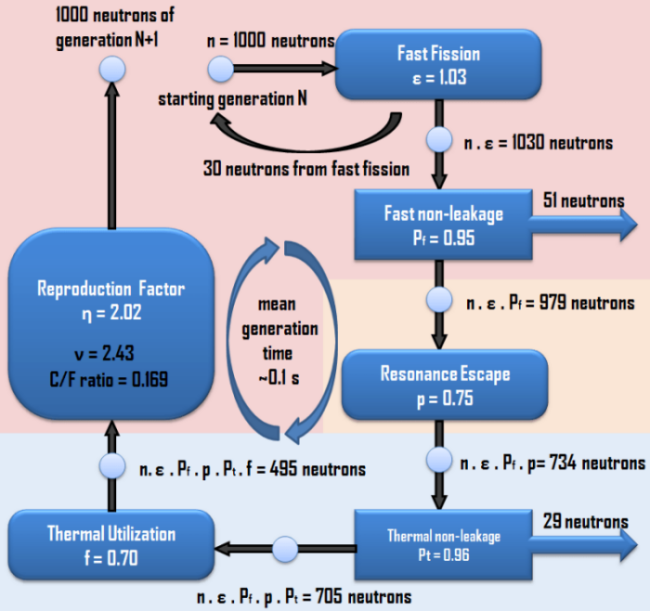
\includegraphics[width=0.65\textwidth]{neutron.balance.png}
%        \caption{}
    \end{figure}
\end{frame}


\begin{frame}{Neutron consumption = production rates in the critical reactor}
    \begin{enumerate}[series=outerlist,topsep=0pt,itemsep=21pt,leftmargin=*,label=(\arabic*)]
        \item[]$N_M$ -- atoms of fissile material per unit volume
        \item[]$\sigma_M$ -- absorption cross section
        \item[]$N_G, \; \sigma_G$ -- fertile material
        \item[]Fissionable material absorbs only thermal neutrons
        \item[]$N_M\sigma_M\phi$ -- neutron absorption rate by fissionable material
        \item[]$\eta_M N_M\sigma_M\phi$ -- fissions produce fast neutrons
    \end{enumerate}
\end{frame}


\begin{frame}{Production of neutrons also comes from fast fission}
    \begin{enumerate}[series=outerlist,topsep=0pt,itemsep=21pt,leftmargin=*,label=(\arabic*)]
        \item[]Fast fission factor $\epsilon$ defines net rate of production of fast neutrons to production rate of fast neutrons by thermal fission
        \item[]$\epsilon - 1$ -- fast neutrons come from fission of fertile material with fast neutrons
        \item[]$\epsilon\eta_M N_M \sigma_M \phi$ -- production rate of fast neutrons from fission
    \end{enumerate}
\end{frame}


\begin{frame}{Neutrons leak during scatter from the fast region to resonances}
    \begin{enumerate}[series=outerlist,topsep=0pt,itemsep=21pt,leftmargin=*,label=(\arabic*)]
        \item[]$P_F$ -- probability the neutrons do not leak
        \item[]$\epsilon\eta_M N_M\sigma_M\phi P_F$ -- rate fast neutrons do not leak
        \item[]Neutrons can be absorbed in resonance region
        \item[]$p$ -- probability that escape to thermal region
        \item[]$\epsilon\eta_M N_M\sigma_M\phi P_F p$ -- neutrons produced in thermal region
    \end{enumerate}
\end{frame}


\begin{frame}{Finally, thermal neutrons leak}
    \begin{enumerate}[series=outerlist,topsep=0pt,itemsep=21pt,leftmargin=*,label=(\arabic*)]
        \item[]Neutrons complete a cycle as $\epsilon p \eta_M P_F P_T N_M \sigma_M \phi$ reach thermal region per unit volume per time
        \item[]Thermal neutrons are consumed by absorption in fissionable material, nonfissionable material, leakage
        \item[]Absorption in fissionable material leads to regeneration of fission neutrons
    \end{enumerate}
\end{frame}


\begin{frame}{Let's derive the neutron balance in the critical reactor}
    \begin{enumerate}[series=outerlist,topsep=0pt,itemsep=21pt,leftmargin=*,label=(\arabic*)]
        \item[]Assume representative unit volume
        \item[]$N_M$ -- atoms of single fissile species with absorption cross section $\sigma_M$
        \item[]$N_G$ -- atoms of single fertile material with absorption cross section $\sigma_G$
        \item[]Same for coolant, moderator, structure (lumped together)
        \item[]Control absorbers
        \item[]Assume steady state amounts of Xe, Sm
    \end{enumerate}
\end{frame}


\begin{frame}{Rate of thermal neutron production = consumption for initial loading}
    \begin{equation}
        \eta_M \epsilon p P_F P_T N_M \sigma_M \phi = DB^2\phi + N_M\sigma_M\phi + N_G\sigma_G\phi + \sum_P N_P\sigma_P\phi +  N_{Xe}\sigma_{Xe}\phi + N_{Sm}\sigma_{Sm}\phi + N_E\sigma_E\phi
    \end{equation}
\end{frame}


\begin{frame}{For the operating reactor, it is slightly more complicated}
    \begin{equation}
        \footnotesize
        \begin{aligned}
            & \sum_M\eta_M \epsilon p P_F P_T N_M \sigma_M \phi = 
            \\
            & DB^2\phi +  \newline \sum_MN_M\sigma_M\phi +  \sum_HN_H\sigma_H\phi +  \sum_P N_P\sigma_P\phi +  \sum_FN_F\sigma_F\phi +  N_G\sigma_G\phi +  N_{Xe}\sigma_{Xe}\phi +  N_{Sm}\sigma_{Sm}\phi +  N_E\sigma_E\phi
        \end{aligned}
    \end{equation}

    \vspace*{\fill}

    \begin{enumerate}[series=outerlist,topsep=0pt,itemsep=21pt,leftmargin=*,label=(\arabic*)]
        \item[]Production = sum of all fissionable species
        \item[]H = nonfissionable higher isotopes (U-236, etc.)
        \item[]F = fission products lower than Xe, Sm
        \item[]\href{https://piazza.com/class_profile/get_resource/ll13mxo3tb15l/ll1g94jnkby5jr}{Benedict notes}
    \end{enumerate}
\end{frame}


\begin{frame}{We can calculate burnup by deriving composition changes in time}
    \begin{equation}
        \LARGE
        \frac{dN_{25}}{dt}=-N_{25}\sigma_{25}\phi(t)
    \end{equation}
    
    \begin{equation}
        \LARGE
        N_{25}=N_{25}^0e^{-\sigma_{25}\int_0^t\phi dt'}
    \end{equation}
    
    \begin{equation}
        \LARGE
        \theta \equiv \int_0^t\phi(t')dt'\rightarrow \theta = \overline{\phi} t
    \end{equation}

    \begin{equation}
        \LARGE
        N_{25}=N_{25}^0e^{-\sigma_{25}\theta}
    \end{equation}
\end{frame}


\begin{frame}{Flux time expresses extent of exposure to irradiation}
    \begin{enumerate}[series=outerlist,topsep=0pt,itemsep=21pt,leftmargin=*,label=(\arabic*)]
        \item[]Defined in units of neutrons per square centimeter
        \item[]Also called fluence
        \item[]Typically if flux is $10^{14} \; n/cm^2/s$ and $10^7 \; s$
        \item[]Then flux time is on the order of $10^{21} \; n/cm^2$
        \item[]So they call that neutrons per kilobarn because of course they do
    \end{enumerate}
\end{frame}


\begin{frame}{U-236 is produced by capture in U-235}
    \begin{equation}
        \LARGE
        \frac{dN_{26}}{dt}=\frac{\alpha_{25}}{1 + \alpha_{25}}\cdot N_{25}\sigma_{25}\phi-N_{26}\sigma_{26}\phi
    \end{equation}
    
    \begin{equation}
        \LARGE
        \alpha \equiv \frac{\sigma_A}{\sigma_F}
    \end{equation}
    
    \begin{equation}
        \LARGE
        \frac{1}{1+\alpha} = \frac{\sigma_F}{\sigma_F+\sigma_A}
    \end{equation}

    \begin{equation}
        \LARGE
        \frac{\alpha}{1+\alpha}=\frac{\sigma_A}{\sigma_F} \cdot \frac{\sigma_F}{\sigma_F+\sigma_A} =\frac{\sigma_A}{\sigma_F+\sigma_A}
    \end{equation}

    \begin{equation}
        \LARGE
        N_{26}=\frac{N_{25}^0\sigma_{25}\alpha_{25}}{(\sigma_{25}-\sigma_{26})(1 + \alpha_{25})}\cdot(e^{-\sigma_{26}\theta}-e^{-\sigma_{25}\theta})
    \end{equation}
\end{frame}


\begin{frame}{Pu-239 production is more complicated}
    \begin{enumerate}[series=outerlist,topsep=0pt,itemsep=21pt,leftmargin=*,label=(\arabic*)]
        \item[]$\frac{dN_{49}}{dt} = $
        \item[]$+ N^0_{28}\sigma_{28}\phi$ -- production from thermal neutron absorption in U-238
        \item[]$+ \eta_{X}\epsilon P_F (1-p) N_{X}\sigma_{X}\phi$ -- fission neutrons from X absorbed by Y in the resonance region 
        \item[]$- N_{49}\sigma_{49}\phi$ -- thermal neutron absorption in Pu-239
        \item[]$+ \frac{\alpha_{28}}{1 + \alpha_{28}}\cdot\frac{\epsilon-1}{\eta_{28-1}}(\eta_{25}N_{25}\sigma_{25} + \eta_{49}N_{49}\sigma_{49} + \eta_{41}N_{41}\sigma_{41})\phi$ -- fast neutron absorption
    \end{enumerate}
\end{frame}


\begin{frame}{Net formation can be simplified with flux time}
    \begin{equation}
        \LARGE
        \frac{dN_{49}}{d\theta}=N_{28}^0\sigma_{28} + \kappa_{25}N_{25}\sigma_{25}-\gamma_{49}N_{49}\sigma_{49} + \kappa_{41}N_{41}\sigma_{41}
    \end{equation}
    
    \begin{equation}
        \LARGE
        \kappa_m \equiv\eta_m\epsilon P_F(1-p) + \eta_m\frac{\alpha_{28}}{1 + \alpha_{28}}\cdot\frac{\epsilon-1}{\eta_{28}-1}
    \end{equation}
    
    \begin{equation}
        \LARGE
        \gamma_{49} = 1 - \kappa_{49}
    \end{equation}
\end{frame}


\begin{frame}{The remaining isotopes of plutonium produced are Pu-242, Pu-241, Pu-240}
    \begin{equation}
        \LARGE
        \frac{dN_{42}}{d\theta}=\frac{\alpha_{41}}{1 + \alpha_{41}}\cdot N_{41}\sigma_{41}-N_{42}\sigma_{42}
    \end{equation}
    
    \begin{equation}
        \LARGE
        \frac{dN_{41}}{d\theta}=N_{40}\sigma_{40}-N_{41}\sigma_{41}
    \end{equation}
    
    \begin{equation}
        \LARGE
        \frac{dN_{40}}{d\theta}=\frac{\alpha_{49}}{1 + \alpha_{49}}N_{49}\sigma_{49}-N_{40}\sigma_{40}
    \end{equation}
\end{frame}


\begin{frame}{An exact solution can be solved analytically, but why bother}
    \begin{enumerate}[series=outerlist,topsep=0pt,itemsep=7pt,leftmargin=*,label=(\arabic*)]
        \item[]Formation of Pu-239 by absorption of resonance neutrons from Pu-241 can be neglected
    \end{enumerate}

    \vspace*{\fill}

    \begin{equation}
        \LARGE
        \kappa_{41} N_{41} \sigma_{41} << \gamma_{41} N_{49} \sigma_{49}
    \end{equation}
    
    \begin{equation}
        \LARGE
        \frac{dN_{49}}{d\theta}=N_{28}^0\sigma_{28} + \kappa_{25} N_{25}\sigma_{25}-\gamma_{49} N_{49} \sigma_{49}
    \end{equation}
    
    \begin{equation}
        \LARGE
        N_{49}(0) = 0
    \end{equation}
\end{frame}


\begin{frame}{Fission products are produced by $^{235}U$}
    \begin{equation}
        \LARGE
        \frac{dN_{25}^F}{d\theta}=\frac{1}{1 + \alpha_{25}}\cdot N_{25}\sigma_{25}
    \end{equation}
    
    \begin{equation}
        \LARGE
        N_{25}^F(0)=0
    \end{equation}
\end{frame}


\begin{frame}{Fission products also from $^{239}Pu$}
    \begin{equation}
        \LARGE
        \frac{dN_{49}^F}{d\theta}=\frac{1}{1 + \alpha_{49}}\cdot N_{49}\sigma_{49}
    \end{equation}
    
    \begin{equation}
        \LARGE
        N_{49}^F(0)=0
    \end{equation}
\end{frame}


\begin{frame}{And from $^{241}Pu$}
    \begin{equation}
        \LARGE
        \frac{dN_{41}^F}{d\theta}=\frac{1}{1 + \alpha_{41}}\cdot N_{41}\sigma_{41}
    \end{equation}
    
    \begin{equation}
        \LARGE
        N_{41}^F(0)=0
    \end{equation}
\end{frame}


\begin{frame}{The Pu solutions can be checked by an overall neutron balance}
    \begin{equation}
        \LARGE
        \alpha_{49} N_{49}^F=N_{40} + N_{41} + N_{42} + N_{41}^F
    \end{equation}
\end{frame}


\begin{frame}{Burnup can be computed as a function of the neutron balance}
    \begin{enumerate}[series=outerlist,topsep=0pt,itemsep=7pt,leftmargin=*,label=(\arabic*)]
        \item[]Fission energy is about 200 MeV per U-235 atom fissioned
        \item[]About $9.5 \times 10^5 \; MWD/MTU$
    \end{enumerate}

    \vspace*{\fill}

    \begin{equation}
        \LARGE
        B=9.5 \times 10^5 \cdot w
    \end{equation}
    
    \begin{equation}
        \LARGE
        w \equiv \frac{235\cdot N_{25}^F + 238\cdot N_{28}^F + 239\cdot N_{49}^F  + 241\cdot N_{41}^F}{235\cdot N_{25}^0 + 238\cdot N_{28}^0}
    \end{equation}

    \vspace*{\fill}

    \begin{enumerate}[series=outerlist,topsep=0pt,itemsep=7pt,leftmargin=*,label=(\arabic*)]
        \item[]Pu accumulation can be plotted as a function of burnup
    \end{enumerate}
\end{frame}


\begin{frame}{U-238 continuously depletes during operation}
    \begin{equation}
        \Large
        N_{28}(\theta)=N_{28}^0-N_{28}^0\sigma_{28}\theta-\kappa_{25}(1 + \alpha_{28})N_{25}^F-\kappa_{49}(1 + \alpha_{49})N_{49}^F-N_{28}^F
    \end{equation}
    
    \vspace*{\fill}

    \begin{enumerate}[series=outerlist,topsep=0pt,itemsep=21pt,leftmargin=*,label=(\arabic*)]
        \item[]Initial amount of atoms U-238
        \item[]Absorption of thermal neutrons
        \item[]Absorption of resonance,fast neutrons from U-235 fission
        \item[]Absorption of resonance,fast neutrons from Pu-239 fission
        \item[]Loss due to fast fission of U-238
    \end{enumerate}
\end{frame}


\begin{frame}{The overall neutron balance can be checked}
    \begin{equation}
        \LARGE
        N_{28}=N_{28}^0-N_{28}^F-N_{49}-N_{49}^F-N_{40}-N_{41}-N_{41}^F-N_{42}
    \end{equation}
\end{frame}


\begin{frame}[plain]{}
    \centering\LARGE\textbf{Fisson product production}
\end{frame}


\addtocounter{framenumber}{-1} 
\begin{frame}{Fission product atoms can be determined from the number of fissions}
    \begin{equation}
        \LARGE
        N_i(t) = Y_{25}^iN_{25}^F + Y_{49}^iN_{49}^F
    \end{equation}
    
    \vspace*{\fill}

    \begin{enumerate}[series=outerlist,topsep=0pt,itemsep=21pt,leftmargin=*,label=(\arabic*)]
        \item[]$N_i(t)$ -- number of $i$ fission product atoms
        \item[]$N_m^F$ -- number of $m$ atoms fissioned
        \item[]$Y_m^i$ cumulative yield of $i$ fission product atom by thermal fission of $m$
        \item[]Cumulative fission is the fraction of fissions that directly yield the isotope and its precursors
        \item[]Sum of the direct yields of the nuclide and decay precursors
    \end{enumerate}
\end{frame}


\begin{frame}{}
    \begin{figure}
        \centering
        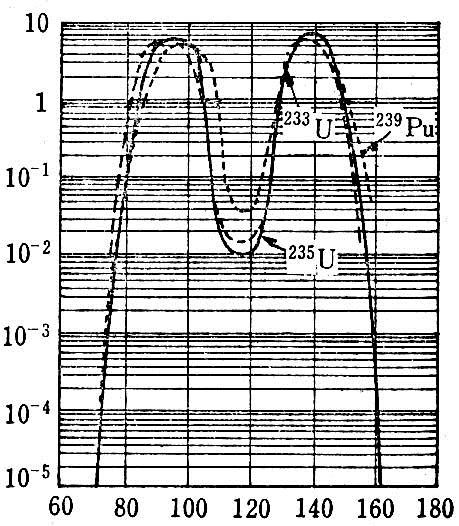
\includegraphics[width=0.50\textwidth]{the-fission.yield.jpg}
%        \caption{}
    \end{figure}
\end{frame}


\begin{frame}{The fission product production equations can be modified}
    \begin{equation}
        \LARGE
        \frac{N_{25}^F}{dt}=N_{25} \sigma_{25}^{fission} \overline{\phi}
    \end{equation}
    
    \begin{equation}
        \LARGE
        \frac{N_{49}^F}{dt}=N_{49} \sigma_{49}^{fission} \overline{\phi}
    \end{equation}
    
    \vspace*{\fill}

    \begin{enumerate}[series=outerlist,topsep=0pt,itemsep=21pt,leftmargin=*,label=(\arabic*)]
        \item[]Neglect absorption in fission products and precursors
        \item[]For $t > T$, no fission
    \end{enumerate}
\end{frame}


\begin{frame}{Individual fission product atom production can be obtained}
    \begin{equation}
        \LARGE
        \begin{aligned}
            \frac{dN_i}{dt} & = Y_{25}^i N_{25}\sigma_{25}^f\overline{\phi} + Y_{49}^i N_{49}\sigma_{49}^f\overline{\phi}-\lambda_iN_i
            \\
            & t < T
        \end{aligned}
    \end{equation}
    
    \begin{equation}
        \LARGE
        \begin{aligned}
            \frac{dN_i}{dt} & = -\lambda_iN_i
            \\
            & t > T
        \end{aligned}
    \end{equation}
\end{frame}


\begin{frame}{With post irradiation cooling}
    \begin{enumerate}[series=outerlist,topsep=0pt,itemsep=21pt,leftmargin=*,label=(\arabic*)]
        \item[]Cooling time -- C
    \end{enumerate}
    
    \vspace*{\fill}

    \begin{equation}
        \Large
        N_i(T + C)=e^{-\lambda_iC}\int_0^Te^{-\lambda_i(T-t)} (Y_{25}^iN_{25}\sigma_{25}^f\overline{\phi} + Y_{49}^iN_{49}\sigma_{49}^f\overline{\phi})dt
    \end{equation}
    
    \vspace*{\fill}

    \begin{enumerate}[series=outerlist,topsep=0pt,itemsep=21pt,leftmargin=*,label=(\arabic*)]
        \item[]With long lived nuclides, which are most important anyway
    \end{enumerate}
    
    \vspace*{\fill}

    \begin{equation}
        \LARGE
        N_i(T + C)=e^{-\lambda_iC}\int_0^T (Y_{25}^iN_{25}\sigma_{25}^f\overline{\phi} + Y_{49}^iN_{49}\sigma_{49}^f\overline{\phi})dt
    \end{equation}
    
    \vspace*{\fill}

    \begin{enumerate}[series=outerlist,topsep=0pt,itemsep=21pt,leftmargin=*,label=(\arabic*)]
        \item[]By definition
    \end{enumerate}
    
    \vspace*{\fill}

    \begin{equation}
        \LARGE
        N_i(T + C)=e^{-\lambda_iC}[Y_{25}^iN_{25}^F(T) + Y_{49}^iN_{49}^F(T)]
    \end{equation}
\end{frame}


\begin{frame}[plain]{}
    \centering\LARGE\textbf{Radioactivity from neutron activation}
\end{frame}


\addtocounter{framenumber}{-1} 
\begin{frame}{Tritium is produced in reactors by neutron reaction with Li, B, deuterium}
    \begin{enumerate}[series=outerlist,topsep=0pt,itemsep=7pt,leftmargin=*,label=(\arabic*)]
        \item[]Also can be designed to produce tritium by irradiating Li targets with thermal neutrons
    \end{enumerate}
    
    \vspace*{\fill}

    \begin{equation*}
        ^6_3Li+^1_0n \rightarrow ^4_2He+^3_1H
    \end{equation*}
    
    \vspace*{\fill}

    \begin{enumerate}[series=outerlist,topsep=0pt,itemsep=7pt,leftmargin=*,label=(\arabic*)]
        \item[]Neutron activation of boron produces Li and He
        \item[]Thermal cross section 3837 b
    \end{enumerate}
    
    \vspace*{\fill}

    \begin{equation*}
        ^{10}_5B+^1_0n \rightarrow ^7_3Li+^4_2He
    \end{equation*}
    
    \vspace*{\fill}

    \begin{enumerate}[series=outerlist,topsep=0pt,itemsep=7pt,leftmargin=*,label=(\arabic*)]
        \item[]Fast spectrum
        \item[]Super small cross section; negligible
    \end{enumerate}
    
    \vspace*{\fill}

    \begin{equation*}
        \begin{aligned}
            ^{10}_5B+^1_0n & \rightarrow 2 ^4_2He+^3_1H
            \\
            ^{11}_5B+^1_0n & \rightarrow ^9_4Be+^3_1H
        \end{aligned}
    \end{equation*}
\end{frame}


\begin{frame}{In \acsp{pwr} boron is dissolved in coolant for long-term reactivity control}
    \begin{enumerate}[series=outerlist,topsep=0pt,itemsep=21pt,leftmargin=*,label=(\arabic*)]
        \item[]Concentration change occurs over short time period short compared to half-life of tritium
        \item[]Boron concentrations are repeated over each cycle
        \item[]Assume an average concentration
        \item[]$i$ = atoms of species $i$ producing tritium
    \end{enumerate}
    
    \vspace*{\fill}

    \begin{equation}
        \LARGE
        N_T\lambda_T=\sum_i N_i\sigma_i\phi(1-e^{-\lambda_T T})
    \end{equation}
\end{frame}


\begin{frame}{C-14 formed in reactors from activation of nitrogen}
    \begin{enumerate}[series=outerlist,topsep=0pt,itemsep=11pt,leftmargin=*,label=(\arabic*)]
        \item[]Residual nitrogen impurity in oxide fuel
        \item[]Air dissolved in coolant
        \item[]$^{14}_7N+^1_0n \rightarrow ^{14}_6C+^1_1H$ 
        \item[]2 b cross section though
        \item[]$^{17}_8O+^1_0n \rightarrow ^{14}_6C+^4_2He$
        \item[]0.03\% of natural oxygen
        \item[]0.2 b 
    \end{enumerate}
    
    \vspace*{\fill}

    \begin{equation}
        \LARGE
        N_C\lambda_C=\lambda_CT\sum_i N_i \sigma_i \phi
    \end{equation}
\end{frame}




























































\begin{frame}[plain]{}
    \begin{figure}
        \centering
        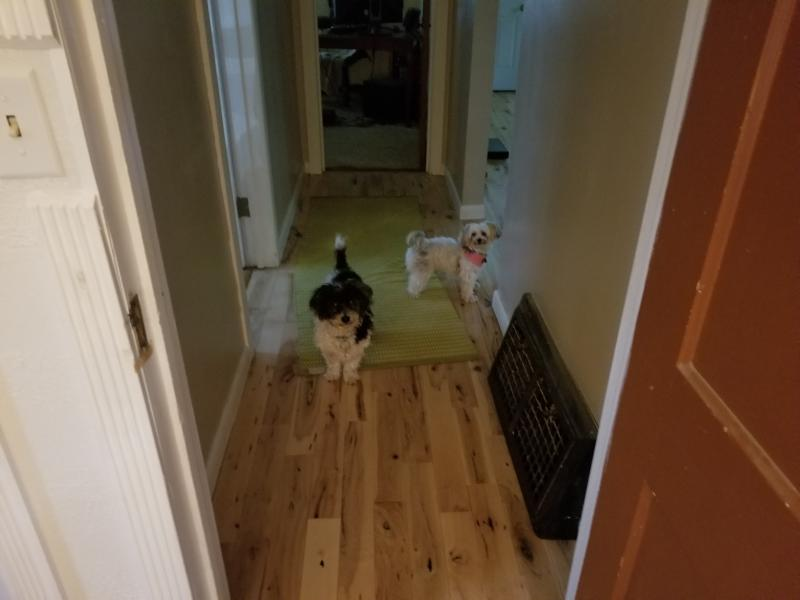
\includegraphics[width=0.75\textwidth]{final.jpg}
%        \caption{}
    \end{figure}
\end{frame}


%%%%%%%
%\begin{frame}{}
%    \begin{columns}
%
%        \begin{column}{0.50\textwidth}
%            \begin{enumerate}[series=outerlist,topsep=0pt,itemsep=21pt,leftmargin=*,label=(\arabic*)]
%                \item[]
%                \item[]
%            \end{enumerate}
%        \end{column}
%
%        \begin{column}{0.50\textwidth}
%            \begin{enumerate}[series=outerlist,topsep=0pt,itemsep=21pt,leftmargin=*,label=(\arabic*)]
%                \item[]
%                \item[]
%            \end{enumerate}
%        \end{column}
%
%    \end{columns}
%\end{frame}

%    \begin{figure}
%        \centering
%        \includegraphics[width=0.75\textwidth]{wsc.png}
%        \caption{\acs{wsc}}
%    \end{figure}


%\begin{frame}{References}
%    \bibliographystyle{nsf}
%    \footnotesize
%    \bibliography{references}
%\end{frame}
%%%%%%%


\end{document}
